\documentclass[a4paper,12pt,oneside]{report}
\usepackage[english]{learningnotes}
\usepackage{needspace}
\newcommand{\exerciseheading}[1]{%
  \par\Needspace{5\baselineskip}\noindent\textbf{#1}\par\nobreak}
\newcommand{\solutionheading}[1]{%
  \par\Needspace{5\baselineskip}\noindent
  \begingroup\setlength{\fboxsep}{1pt}%
  \colorbox{yellow}{\strut\textbf{#1}}\endgroup\par\nobreak}

\notestitle{FSL}
\notessubtitle{Fundamentals of statistical learning}
\notesauthor{Matteo}
\notesdate{\today}

\begin{document}

\makenotestitle
\notescontents

\chapter{Probability}

\section{Why probability?}

Observed data are the results of processes whose behavior we may not fully
know. To reason about them, we describe the process with a probabilistic
model. Probability lets us work forward from a model to possible outcomes;
statistical inference uses observed outcomes to learn about the model.

\begin{framedexample}{A coin toss}
Let $\theta=P(\text{heads})$ be the probability that a coin lands heads.
If $\theta$ is known, we can ask how likely it is to observe three heads
in five tosses. If instead we observe three heads in five tosses while
$\theta$ is unknown, we can use those data to learn about $\theta$.
\end{framedexample}

\section{Sample spaces and events}

Before assigning probabilities, we must specify what the experiment can
produce. We start with a finite set of possible results.

\begin{frameddefn}{Outcomes and events}\label{def:outcomes-events}
A random experiment is a process whose result is not known in advance.
Each possible result is an \emph{outcome} $\omega$. The set of all possible
outcomes is the \emph{sample space} $\Omega$. An \emph{event} is a subset
$A\subseteq\Omega$; it occurs when the observed outcome belongs to $A$.
\end{frameddefn}

\begin{framedexample}{Rolling a die}\label{ex:die-events}
For one roll of a six-sided die, the sample space is
$\Omega=\{1,2,3,4,5,6\}$. The event ``the result is even'' is
$A=\{2,4,6\}$. The whole sample space $\Omega$ is the certain event,
while $\varnothing$ is the impossible event.
\end{framedexample}

\subsection{Operations on events}

Events are subsets of the same sample space $\Omega$, so set operations
let us describe new events in terms of $A$ and $B$:

\begin{itemize}
  \item \textbf{Union:}
  $A\cup B=\{\omega\in\Omega:\omega\in A\text{ or }\omega\in B\}$.
  This event occurs when at least one of $A$ and $B$ occurs;
  ``or'' includes the case in which both occur.
  In particular, $A\cup\varnothing=A$ and $A\cup\Omega=\Omega$.

  \item \textbf{Intersection:}
  $A\cap B=\{\omega\in\Omega:\omega\in A\text{ and }\omega\in B\}$.
  This event occurs when both $A$ and $B$ occur.
  In particular, $A\cap\Omega=A$ and $A\cap\varnothing=\varnothing$.

  \item \textbf{Complement:}
  $A^c=\Omega\setminus A
       =\{\omega\in\Omega:\omega\notin A\}$.
  This event occurs when $A$ does not occur.
  In particular, $A\cup A^c=\Omega$ and $A\cap A^c=\varnothing$.
\end{itemize}

For the die in Example~\ref{ex:die-events}, let
$B=\{4,5,6\}$ be the event ``the result is at least four''. Then
$A\cup B=\{2,4,5,6\}$, $A\cap B=\{4,6\}$, and
$A^c=\{1,3,5\}$.

Two events are \emph{disjoint} when $A\cap B=\varnothing$, so they
cannot occur together. If $A\subseteq B$, every outcome in $A$ is
also in $B$: whenever $A$ occurs, $B$ occurs.

\begin{framedprop}{De Morgan's laws}\label{prop:de-morgan}
For any events $A$ and $B$,
\[
  (A\cup B)^c=A^c\cap B^c,
  \qquad
  (A\cap B)^c=A^c\cup B^c.
\]
More generally, for events $A_1,\ldots,A_n$,
\[
  \left(\bigcup_{i=1}^{n}A_i\right)^c
    =\bigcap_{i=1}^{n}A_i^c,
  \qquad
  \left(\bigcap_{i=1}^{n}A_i\right)^c
    =\bigcup_{i=1}^{n}A_i^c.
\]
\end{framedprop}

The first identity says that ``none occurs'' means that every event
fails. The second says that ``not all occur'' means that at least one
event fails. We will use the second identity in the proof of
Bonferroni's inequality.

\subsection{Partitions and event decomposition}

A useful way to study an event is to split it into disjoint pieces. For
any events $A$ and $B$, exactly one of $B$ and $B^c$ occurs, so
\[
  A=A\cap\Omega
   =A\cap(B\cup B^c)
   =(A\cap B)\cup(A\cap B^c).
\]
The two events on the right are disjoint. For example, a car can fail
an emissions test either while it pollutes or while it does not.

More generally, a \emph{partition} $B_1,\ldots,B_n$ of $\Omega$ consists
of pairwise disjoint events whose union is $\Omega$. Every event $A$
can then be written as
\[
  A=\bigcup_{i=1}^{n}(A\cap B_i),
  \qquad
  (A\cap B_i)\cap(A\cap B_j)=\varnothing\quad(i\neq j).
\]
This decomposition will let us add the probabilities of different
ways in which the same event can occur.

\clearpage
\section{Probability}

There are several ways to interpret a probability. Under a
\emph{symmetry} assumption, equally likely outcomes give
$P(A)=|A|/|\Omega|$. A \emph{frequency} interpretation concerns the
long-run proportion of repetitions in which $A$ occurs. A
\emph{subjective} interpretation expresses a degree of belief about
$A$. The axioms below state the mathematical rules that a probability
assignment must satisfy, regardless of its interpretation.

\begin{framedexample}{Two dice}
If the $36$ ordered results of rolling two dice are equally likely,
they form the sample space $\Omega=\{1,\ldots,6\}^2$. The sum is eight for
$(2,6),(3,5),(4,4),(5,3),(6,2)$, so the probability of that event is
$5/36$. Counting outcomes this way is valid because the ordered pairs
are equally likely.
\end{framedexample}

\begin{frameddefn}{Probability on a finite sample space}\label{def:probability-finite}
A probability measure $P$ assigns a number $P(A)$ to every event
$A\subseteq\Omega$ such that:
\begin{enumerate}
  \item $0\leq P(A)\leq 1$ for every event $A$;
  \item $P(\Omega)=1$;
  \item if $A\cap B=\varnothing$, then
        $P(A\cup B)=P(A)+P(B)$.
\end{enumerate}
The last property is called \emph{finite additivity}.
\end{frameddefn}

Because $A$ and $A^c$ are disjoint and their union is $\Omega$,
these axioms give $P(A^c)=1-P(A)$. In particular,
$P(\varnothing)=0$. 

They also imply \emph{monotonicity}: if
$A\subseteq B$, then $B=A\cup(B\cap A^c)$ is a disjoint union,
so $P(B)=P(A)+P(B\cap A^c)\geq P(A)$.

\begin{framedexample}{A fair die}
If the six outcomes of a die roll are equally likely, each has
probability $1/6$. The event $A=\{2,4,6\}$ therefore has probability
$P(A)=3/6=1/2$.
\end{framedexample}

For an infinite sample space, finite additivity is replaced by
\emph{countable additivity}: for pairwise disjoint events
$A_1,A_2,\ldots$,
\[
  P\!\left(\bigcup_{i=1}^{\infty}A_i\right)
    =\sum_{i=1}^{\infty}P(A_i).
\]
In that setting, a probability measure is defined on a suitable
family of events rather than necessarily on every subset of
$\Omega$. On a finite sample space, the finite formulation above is
enough.

\subsection{Inclusion--exclusion}

Finite additivity directly handles disjoint events. If $A$ and $B$
overlap, adding $P(A)$ and $P(B)$ counts their intersection twice.

\begin{framedprop}{Inclusion--exclusion for two events}
For any events $A$ and $B$,
\[
  P(A\cup B)=P(A)+P(B)-P(A\cap B).
\]
\end{framedprop}

\begin{proof}
Split $A\cup B$ into the disjoint events $A$ and $B\cap A^c$:
\[
  P(A\cup B)=P(A)+P(B\cap A^c).
\]
The event $B$ is itself the disjoint union of $A\cap B$ and
$A^c\cap B$. Thus
$P(B\cap A^c)=P(B)-P(A\cap B)$, which gives the formula.
\end{proof}

\begin{framedexample}{Overlapping die events}
Let $A=\{2,4,6\}$ and $B=\{4,5,6\}$. Then
$P(A)=P(B)=1/2$ and $P(A\cap B)=1/3$. Therefore
\[
  P(A\cup B)=\frac12+\frac12-\frac13=\frac23,
\]
in agreement with $A\cup B=\{2,4,5,6\}$.
\end{framedexample}

Applying the two-event formula twice gives the three-event version:
\[
\begin{aligned}
P(A\cup B\cup C)
  ={}&P(A)+P(B)+P(C)\\
    &-P(A\cap B)-P(A\cap C)-P(B\cap C)\\
    &+P(A\cap B\cap C).
\end{aligned}
\]
The final term restores outcomes in all three events: they were
added three times and subtracted three times.

For $n$ events, the same pattern continues:
\[
  P\!\left(\bigcup_{i=1}^{n}A_i\right)
  =\sum_{\varnothing\neq I\subseteq\{1,\ldots,n\}}
     (-1)^{|I|+1}P\!\left(\bigcap_{i\in I}A_i\right).
\]
To see why, consider an outcome contained in exactly $k$ of the
events. It is counted $\binom{k}{j}$ times among the intersections
of size $j$, so its total coefficient on the right is
$\sum_{j=1}^{k}(-1)^{j+1}\binom{k}{j}=1$. An outcome in none of the
events contributes zero to both sides.

\subsection{Probability bounds}

Sometimes the probabilities of intersections are unknown. We can
still bound the probability of a union.

\begin{framedprop}{Union bound (Boole's inequality)}
For events $A_1,\ldots,A_n$,
\[
  P\!\left(\bigcup_{i=1}^{n} A_i\right)
  \leq \sum_{i=1}^{n}P(A_i).
\]
\end{framedprop}

\begin{proof}
We prove the bound by induction on the number of events.

\textbf{Base case ($n=1$).} The union contains only $A_1$, so the
inequality is an equality: $P(A_1)=\sum_{i=1}^{1}P(A_i)$.

\textbf{Inductive step.} Assume the bound holds for $n$ events and set
$U_n=\bigcup_{i=1}^{n}A_i$. The union of $n+1$ events is
$U_n\cup A_{n+1}$. Applying inclusion--exclusion gives
\[
\begin{aligned}
P\!\left(\bigcup_{i=1}^{n+1}A_i\right)
 &=P(U_n)+P(A_{n+1})-P(U_n\cap A_{n+1})\\
 &\leq P(U_n)+P(A_{n+1})\\
 &\leq \sum_{i=1}^{n}P(A_i)+P(A_{n+1})
  =\sum_{i=1}^{n+1}P(A_i).
\end{aligned}
\]
The first inequality uses $P(U_n\cap A_{n+1})\geq0$; the second uses
the induction hypothesis. Thus the bound holds for every $n\geq1$.
\end{proof}

For a countable sequence, the same inequality follows by applying
the finite bound to the first $n$ events and taking the limit.

\begin{framedprop}{Bonferroni's inequality}
For events $A_1,\ldots,A_n$,
\[
  P\!\left(\bigcap_{i=1}^{n} A_i\right)
  \geq \sum_{i=1}^{n}P(A_i)-(n-1).
\]
\end{framedprop}

\begin{proof}
The second $n$-event form of De Morgan's law turns the complement of
an intersection into a union of complements. Then the union bound gives
\[
\begin{aligned}
P\!\left(\bigcap_{i=1}^{n}A_i\right)
 &=1-P\!\left(\bigcup_{i=1}^{n}A_i^c\right)\\
 &\geq1-\sum_{i=1}^{n}P(A_i^c)\\
 &=1-\sum_{i=1}^{n}(1-P(A_i))
  =\sum_{i=1}^{n}P(A_i)-(n-1).
\end{aligned}
\]
\end{proof}

\subsection{Application: a randomized identity test}

Suppose $F$ and $G$ are polynomials of degree at most $d$. We want to
test whether they are identical without comparing all their coefficients.
Choose a nonempty finite set $S$ of possible evaluation points.

\Needspace{12\baselineskip}
\begin{framedalgo}{Randomized polynomial identity test}\label{alg:identity-test}
Given $F$, $G$, and $S$, report whether the polynomials differ or may
be identical.
\begin{algorithmic}
  \Function{IdentityTest}{$F,G,S$}
    \State Draw $R$ uniformly at random from $S$
    \If{$F(R)\neq G(R)$}
      \State \Return \textsc{different}
    \Else
      \State \Return \textsc{possibly equal}
    \EndIf
  \EndFunction
\end{algorithmic}
\end{framedalgo}

If $F=G$, the test never reports a difference. If $F\neq G$, it fails
to detect the difference only when $R$ belongs to the event
\[
  E=\{r\in S:F(r)=G(r)\}.
\]
Indeed, $E$ contains the roots in $S$ of the nonzero polynomial
$H=F-G$, which has at most $d$ roots. Because $R$ is uniform on $S$,
\[
  P(R\in E)=\frac{|E|}{|S|}\leq\frac{d}{|S|}.
\]
For $S=\{1,\ldots,100d\}$ with $d\geq1$, the probability of missing a
difference is at most $1/100$. The possible error is \emph{one-sided}:
``different'' is certain, while ``possibly equal'' is not a proof of
identity.

\section{Independent events}

\section{Conditional probability}

\section{Bayes' theorem}

\subsection{Odds}

For an event $A$ with $P(A)<1$, its \emph{odds in favor} are
\[
  O(A)=\frac{P(A)}{P(A^c)}
      =\frac{P(A)}{1-P(A)}.
\]
Conversely, $P(A)=O(A)/(1+O(A))$. For a fair die, the odds in
favor of rolling a six are $(1/6)/(5/6)=1/5$, often stated as
one to five. This is different from saying that the probability
is $1/5$; the probability is $1/6$.

\chapter{Crash course exercises}

% Exercise convention: state the problem; define any events used in the
% solution before stating what is sought; show numbered calculation steps;
% cite rules by name without repeating theory; box each final result.
% For multipart problems, state and solve each question separately.

\section{Day 01}

\begin{framedexercise}{Computer virus}
A virus can enter a computer through e-mail or the internet. The
probability of entry through e-mail is $0.30$, through the internet
$0.40$, and through both routes $0.15$. What is the probability that
the virus does not enter at all?
\end{framedexercise}

\solutionheading{Solution.}
Let
\[
  E=\{\text{the virus enters through e-mail}\},\qquad
  I=\{\text{the virus enters through the internet}\}.
\]
\begin{enumerate}[label=\textbf{Step \arabic*:},leftmargin=*]
  \item \textbf{Define the target event.} Let $N=E^c\cap I^c$ be the
  event that the virus does not enter. We seek $P(N)$.
  \item \textbf{Apply De Morgan's law.}
  \[
    P(N)=P\bigl((E\cup I)^c\bigr).
  \]
  \item \textbf{Use the complement rule.}
  \[
    P\bigl((E\cup I)^c\bigr)=1-P(E\cup I).
  \]
  \item \textbf{Calculate the union by inclusion--exclusion.}
  \[
    P(E\cup I)=P(E)+P(I)-P(E\cap I)
      =0.30+0.40-0.15=0.55.
  \]
  \item \textbf{Take the complement.}
  \[
    \boxed{P(N)=1-0.55=0.45=45\%.}
  \]
\end{enumerate}

\Needspace{11\baselineskip}
\begin{framedexercise}{Two children}
A family has two children, and at least one is a boy. What is the
probability that both are boys?
\end{framedexercise}

\solutionheading{Solution.}
Assume each child is independently a boy or a girl with probability
$1/2$. Let
\[
  B_1=\{\text{the first child is a boy}\},\qquad
  B_2=\{\text{the second child is a boy}\}.
\]
\begin{enumerate}[label=\textbf{Step \arabic*:},leftmargin=*]
  \item \textbf{Define the events in the question.} Let
  \begin{align*}
    A&=B_1\cap B_2
       =\{\text{both children are boys}\},\\
    C&=B_1\cup B_2
       =\{\text{at least one child is a boy}\}.
  \end{align*}
  We seek $P(A\mid C)$.
  \item \textbf{List the ordered outcomes.} With $B$ for boy and $G$
  for girl, the equally likely possibilities are
  \[
    \Omega=\{BB,BG,GB,GG\}.
  \]
  \item \textbf{Use the information given.} The event $C$ excludes
  $GG$, leaving
  \[
    C=\{BB,BG,GB\}.
  \]
  \item \textbf{Count the favorable outcomes.} We have $A=\{BB\}$,
  so one of the three outcomes in $C$ is favorable:
  \[
    \boxed{P(A\mid C)=\frac13.}
  \]
\end{enumerate}

\exerciseheading{Check using conditional probability.}
Since $A\subseteq C$, we have $A\cap C=A$. Independence and the
complement rule give
\[
  P(A)=\frac12\cdot\frac12=\frac14,
  \qquad
  P(C)=1-P(\{GG\})=1-\frac14=\frac34.
\]
Therefore
\[
  P(A\mid C)=\frac{P(A\cap C)}{P(C)}
             =\frac{1/4}{3/4}=\frac13.
\]
If the information had instead been \emph{the first child is a boy},
only $BB$ and $BG$ would remain, giving $1/2$. The way the information
is supplied matters.

\clearpage
\section{Day 02}

\begin{framedexercise}{Rolling two dice}
Two fair six-sided dice are rolled. Describe the sample space and
find the probability that their sum is seven.
\end{framedexercise}

\solutionheading{Solution.}
\begin{enumerate}[label=\textbf{Step \arabic*:},leftmargin=*]
  \item \textbf{Write the sample space.} The result is an ordered pair
  $(i,j)$, one value for each die:
  \[
    \Omega=\{(i,j):i,j\in\{1,\ldots,6\}\},
    \qquad |\Omega|=6\cdot6=36.
  \]
  In particular, $(1,6)$ and $(6,1)$ are different outcomes.
  \item \textbf{Define the target event.} Let
  \[
    S=\{(i,j)\in\Omega:i+j=7\}
     =\{(1,6),(2,5),(3,4),(4,3),(5,2),(6,1)\}.
  \]
  We seek $P(S)$, and $|S|=6$.
  \item \textbf{Apply the equally likely outcomes rule.}
  \[
    \boxed{P(S)=\frac{|S|}{|\Omega|}=\frac{6}{36}=\frac16.}
  \]
\end{enumerate}

\Needspace{11\baselineskip}
\begin{framedexercise}{Five-card poker hands}
Assume that all five-card hands from a standard $52$-card deck are
equally likely. Find the probabilities of a flush (five cards of
one suit), four of a kind, and exactly one pair.
\end{framedexercise}

\solutionheading{Solution.}
Because order does not matter, all three probabilities have the same
denominator:
\[
  N=\binom{52}{5}=2\,598\,960.
\]

\exerciseheading{Flush.}
\begin{enumerate}[label=\textbf{Step \arabic*:},leftmargin=*]
  \item \textbf{Choose the suit:} $4$ possibilities.
  \item \textbf{Choose five cards of that suit:} $\binom{13}{5}$
  possibilities.
  \item \textbf{Count and divide:}
  \[
    \boxed{P(\text{flush})
      =\frac{4\binom{13}{5}}{N}
      =\frac{5\,148}{2\,598\,960}
      \approx 0.001981.}
  \]
\end{enumerate}
Under the exercise's definition, this includes straight flushes.

\exerciseheading{Four of a kind.}
\begin{enumerate}[label=\textbf{Step \arabic*:},leftmargin=*]
  \item \textbf{Choose the rank:} $13$ possibilities. All four cards
  of that rank are then fixed.
  \item \textbf{Choose the fifth card:} any of the remaining $48$.
  \item \textbf{Count and divide:}
  \[
    \boxed{P(\text{four of a kind})
      =\frac{13\cdot48}{N}
      =\frac{624}{2\,598\,960}
      \approx 0.0002401.}
  \]
\end{enumerate}

\exerciseheading{Exactly one pair.}
\begin{enumerate}[label=\textbf{Step \arabic*:},leftmargin=*]
  \item \textbf{Choose the pair's rank:} $13$ possibilities.
  \item \textbf{Choose its two suits:} $\binom42$ possibilities.
  \item \textbf{Choose the other three ranks:} $\binom{12}{3}$ ways.
  They must be distinct, avoiding another pair or a triple.
  \item \textbf{Choose their suits:} $4^3$ possibilities.
  \item \textbf{Count and divide:}
  \[
    \boxed{P(\text{exactly one pair})
      =\frac{13\binom42\binom{12}{3}4^3}{N}
      =\frac{1\,098\,240}{2\,598\,960}
      \approx 0.42257.}
  \]
\end{enumerate}
\clearpage
\section{Day 04 (24 sept 26)}

\begin{framedexercise}{Rome and Florence}
The probability that a tourist has visited Rome is $26\%$, the
probability that they have visited Florence is $18\%$, and the
probability that they have visited at least one of the two cities is
$38\%$.

\textbf{Question A.} What is the probability that the tourist has visited
both Rome and Florence?

\textbf{Question B.} What is the probability that the tourist has visited
Rome but not Florence?
\end{framedexercise}

\exerciseheading{Notation.}
Let
\[
  R=\{\text{the tourist has visited Rome}\},\qquad
  F=\{\text{the tourist has visited Florence}\}.
\]
The given probabilities are
\[
  P(R)=0.26,\qquad P(F)=0.18,\qquad P(R\cup F)=0.38.
\]

\solutionheading{Solution to A.}
\begin{enumerate}[label=\textbf{Step \arabic*:},leftmargin=*]
  \item \textbf{Define the target event.} Let
  \[
    A=R\cap F=\{\text{the tourist has visited both cities}\}.
  \]
  We seek $P(A)$.
  \item \textbf{Apply inclusion--exclusion and substitute.}
  \begin{align*}
    P(A)
      &=P(R)+P(F)-P(R\cup F)\\
      &=0.26+0.18-0.38\\
      &=\boxed{0.06=6\%}.
  \end{align*}
\end{enumerate}

\solutionheading{Solution to B.}
\begin{enumerate}[label=\textbf{Step \arabic*:},leftmargin=*]
  \item \textbf{Define the target event.} Let
  \[
    B=R\cap F^c
      =\{\text{the tourist has visited Rome but not Florence}\}.
  \]
  We seek $P(B)$.
  \item \textbf{Subtract the overlap from Rome.}
  \begin{align*}
    P(B)
      &=P(R)-P(A)\\
      &=0.26-0.06\\
      &=\boxed{0.20=20\%}.
  \end{align*}
\end{enumerate}
\Needspace{12\baselineskip}
\begin{framedexercise}{An uncommon disease}
You are diagnosed with an uncommon disease. You know that there is only
a $1\%$ chance of getting it. Let
\[
  D=\{\text{you have the disease}\},\qquad
  T=\{\text{the test is positive}\}.
\]
It is known that the test is imperfect, since
\[
  P(T\mid D)=0.98,\qquad P(T^c\mid D^c)=0.95.
\]

\textbf{Question A.} Given that you test positive, what is the
probability that you have the disease?

\textbf{Question B.} You take the test again, independently of the
first test conditional on whether you have the disease, and it is
positive again. Given both positive results, what is the probability
that you have the disease?
\end{framedexercise}

\solutionheading{Solution to A.}
We seek $P(D\mid T)$. The prior probabilities are $P(D)=0.01$ and
$P(D^c)=0.99$.
\begin{enumerate}[label=\textbf{Step \arabic*:},leftmargin=*]
  \item \textbf{Find the false-positive rate.} By the complement rule,
  \[
    P(T\mid D^c)=1-P(T^c\mid D^c)=1-0.95=0.05.
  \]
  \item \textbf{Find the probability of a positive result.} By the law
  of total probability,
  \begin{align*}
    P(T)
      &=P(T\mid D)P(D)+P(T\mid D^c)P(D^c)\\
      &=0.98\cdot0.01+0.05\cdot0.99\\
      &=0.0593.
  \end{align*}
  \item \textbf{Apply Bayes' theorem.}
  \[
    \boxed{P(D\mid T)
      =\frac{P(T\mid D)P(D)}{P(T)}
      =\frac{0.0098}{0.0593}
      \approx 16.53\%.}
  \]
\end{enumerate}
The positive test raises the probability of disease from $1\%$ to about
$16.53\%$ under the stated assumptions.

\Needspace{20\baselineskip}
\solutionheading{Solution to B.}
Let
\[
  \begin{aligned}
    T_1&=\{\text{the first test is positive}\},\\
    T_2&=\{\text{the second test is positive}\}.
  \end{aligned}
\]
We seek $P(D\mid T_1\cap T_2)$.
\begin{enumerate}[label=\textbf{Step \arabic*:},leftmargin=*]
  \item \textbf{Find the likelihood of two positive results.} Conditional
  independence gives
  \[
    P(T_1\cap T_2\mid D)=0.98^2=0.9604,
    \qquad
    P(T_1\cap T_2\mid D^c)=0.05^2=0.0025.
  \]
  \item \textbf{Find the probability of two positive results.} By the
  law of total probability,
  \begin{align*}
    P(T_1\cap T_2)
      &=P(T_1\cap T_2\mid D)P(D)
        +P(T_1\cap T_2\mid D^c)P(D^c)\\
      &=0.9604\cdot0.01+0.0025\cdot0.99\\
      &=0.012079.
  \end{align*}
  \item \textbf{Apply Bayes' theorem.}
  \[
    \boxed{P(D\mid T_1\cap T_2)
      =\frac{0.9604\cdot0.01}{0.012079}
      \approx 79.51\%.}
  \]
\end{enumerate}
The second positive result raises the probability from about $16.53\%$
to about $79.51\%$ under the conditional independence assumption.
\chapter{Random variables}

\section{From outcomes to data}

Imagine picking one student at random from a class. Before the draw, we do
not know who we will get; afterwards, we can write down that student's
height, weight, and age. Probability describes the draw, while the numbers
we write down are the data.

The possible outcomes form $\Omega$, and $\omega\in\Omega$ is the outcome
that actually occurs. We write $(\Omega,\mathcal F,P)$ for the probability
space: $\mathcal F$ contains the events to which $P$ assigns probabilities.
For a finite $\Omega$, as in Chapter 1, every subset can be an event.

\begin{frameddefn}{Random object}\label{def:random-object}
A \emph{random object} is a measurable map from outcomes to possible
observations:
\[
  Z:\Omega\longrightarrow\mathcal T,
  \qquad \omega\longmapsto Z(\omega).
\]
The set $\mathcal T$ says what kind of thing we record. It could contain
numbers, vectors, images, or text messages. Once $\omega$ is known,
$Z(\omega)$ is the observation we get.
\end{frameddefn}

Think of $Z$ as the rule that turns the outcome into a piece of data.
``Measurable'' is the technical condition that lets us assign a probability
to questions about that data, such as ``is the selected student taller
than $180$ cm?'' It is automatic in our finite examples.

\Needspace{13\baselineskip}
\section{Random variables and random vectors}

Often the observation is a number or a list of numbers. These are two
particularly useful kinds of random objects.

\begin{frameddefn}{Random variable}\label{def:random-variable}
A \emph{random variable} is a measurable map
\[
  X:\Omega\longrightarrow\mathbb R.
\]
It assigns one real number $X(\omega)$ to each outcome $\omega$.
\end{frameddefn}

\begin{center}
  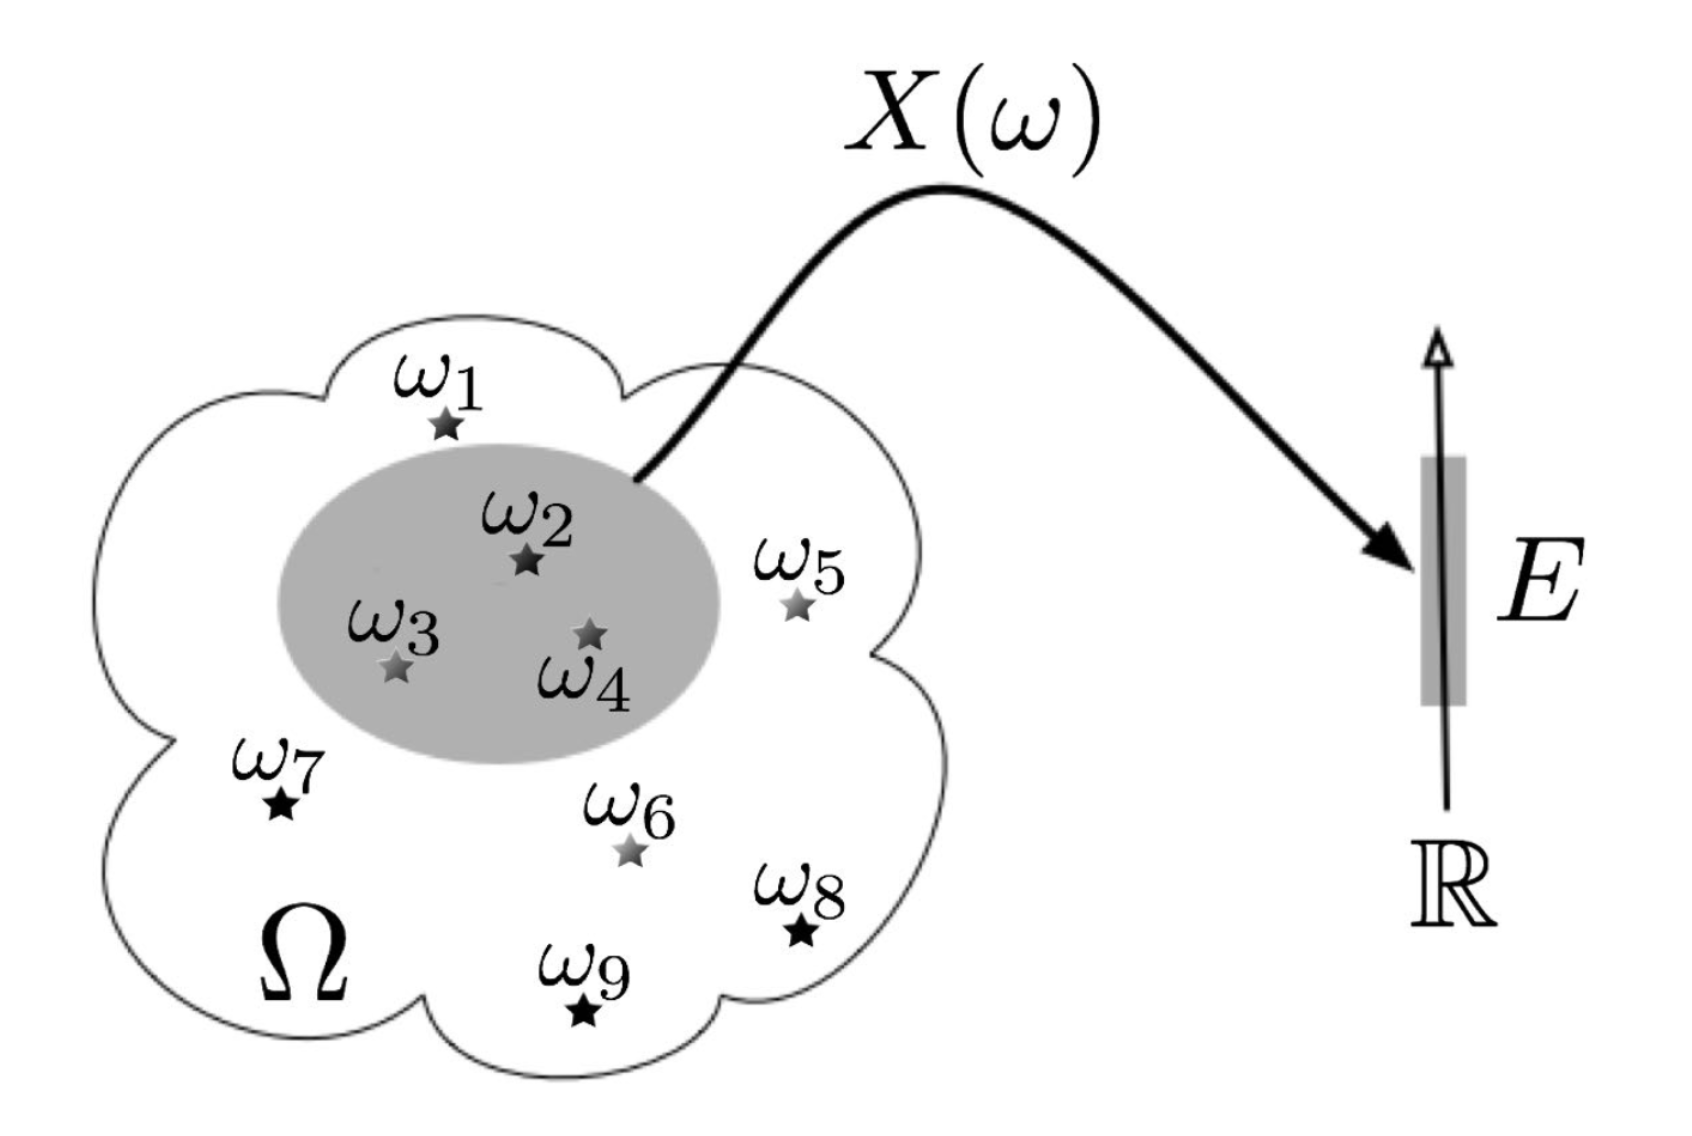
\includegraphics[width=0.65\textwidth]{assets/random-variable-map.png}

  {\small A map from $\Omega$ to $\mathbb R$. Illustration from Brutti's slides.}
\end{center}

\begin{frameddefn}{Random vector}\label{def:random-vector}
A \emph{$p$-dimensional random vector} is a measurable map
\[
  \mathbf X:\Omega\longrightarrow\mathbb R^p,
  \qquad
  \mathbf X(\omega)
    =\bigl(X_1(\omega),\ldots,X_p(\omega)\bigr).
\]
Each coordinate $X_j$ is a real-valued random variable. Thus one
outcome gives us $p$ numbers collected into a vector. These measurements
can be related; they do not have to be independent.
\end{frameddefn}

\Needspace{17\baselineskip}
\begin{framedexample}{One student, one number or three}
Pick a student at random and let $\omega$ identify the student selected.
If $H$ records height in centimetres, then $H(\omega)$ is one number.
For a student who is $178$ cm tall, $H(\omega)=178$.

Now record height $H$, weight $W$ in kilograms, and age $A$ in years for
that \emph{same} student:
\[
  \mathbf X(\omega)
    =\begin{pmatrix}H(\omega)\\W(\omega)\\A(\omega)\end{pmatrix}
    =\begin{pmatrix}178\\72\\21\end{pmatrix}\in\mathbb R^3.
\]
The draw gives us one student, not three. We simply take three
measurements of that student. Before the draw, $H$ and $\mathbf X$ are
uncertain; for the selected student, their values are fixed.
\end{framedexample}

In supervised learning, each sampled item gives us an input $\mathbf X$
(the features) and a target $Y$ (the label or quantity of interest).
Before we see the item, both are uncertain; for an observed item, their
values are fixed.

\begin{framedexample}{House prices}
Choose a house at random. Use its floor area in square metres, number of
rooms, and age in years as features. For a particular house with $85$ m$^2$,
$3$ rooms, and an age of $10$ years, the data look like this:
\[
  \mathbf X(\omega)=(85,3,10),
  \qquad Y(\omega)=240{,}000\ \text{euros}.
\]
The three features make a random vector; the sale price is one random
variable.
\end{framedexample}

\begin{framedexample}{Image labels}
Take a randomly chosen $64\times64$ grayscale photo. Each pixel is one
number from $0$ (black) to $255$ (white). Putting the pixels in a fixed
order gives $\mathbf X(\omega)\in\mathbb R^{4096}$: one vector with
$4096$ entries for one photo. If we set $Y(\omega)=1$ for a cat and
$Y(\omega)=0$ for a dog, then a cat photo gives one feature vector and
the single label $1$. The pixels can be related even though they are
separate coordinates of $\mathbf X$.
\end{framedexample}

\clearpage
\section{Preimages and induced probabilities}

To ask a probability question about the values of $X$, we first find
the outcomes that produce those values.

\begin{frameddefn}{Preimage}\label{def:preimage}
For a random variable $X:\Omega\to\mathbb R$ and a set
$E\subseteq\mathbb R$, the \emph{preimage} (or \emph{inverse image}) of
$E$ is
\[
  X^{-1}(E)=\{\omega\in\Omega:X(\omega)\in E\}\subseteq\Omega.
\]
To find this event, we collect the outcomes whose outputs fall in $E$.
Whenever this set is an event, we write
\[
  P(X\in E)
    =P\bigl(\{\omega\in\Omega:X(\omega)\in E\}\bigr)
    =P\bigl(X^{-1}(E)\bigr).
\]
In particular, for a single value $x$,
\[
  P(X=x)=P\bigl(X^{-1}(\{x\})\bigr).
\]
Here $X$ is the random variable, while $x$ is a particular real number.
\end{frameddefn}

The set $E$ contains values; $X^{-1}(E)$ contains the outcomes that
give those values. In our finite examples, every subset of $\Omega$
is an event.

\Needspace{18\baselineskip}
\begin{framedexample}{Which students have heights in an interval?}
Choose one student uniformly from
$\Omega=\{\text{Anna},\text{Luca},\text{Sara},\text{Marco}\}$.
Let $X$ record height in centimetres:
\[
  \begin{array}{c|rrrr}
    \omega & \text{Anna} & \text{Luca} & \text{Sara} & \text{Marco}\\
    \hline
    X(\omega) & 165 & 178 & 178 & 190
  \end{array}
\]
For $E=[170,180]$, Luca and Sara are the students whose heights fall
inside the interval. Thus
\[
  X^{-1}([170,180])=\{\text{Luca},\text{Sara}\},
  \qquad P(170\leq X\leq180)=\frac24=\frac12.
\]
The same two students also give the exact value $178$:
$X^{-1}(\{178\})=\{\text{Luca},\text{Sara}\}$, so
$P(X=178)=1/2$. One value can correspond to several outcomes.
\end{framedexample}

\Needspace{14\baselineskip}
\begin{framedexample}{Counting heads in two coin tosses}
Toss a fair coin twice, with independent tosses. The four equally
likely outcomes are $\Omega=\{HH,HT,TH,TT\}$, where $H$ means heads
and $T$ means tails. Let $X$ count the heads:
\[
  X(HH)=2,\qquad X(HT)=X(TH)=1,\qquad X(TT)=0.
\]
To get exactly one head, we need either $HT$ or $TH$. Therefore
\[
  X^{-1}(\{1\})=\{HT,TH\},
  \qquad P(X=1)=P(\{HT,TH\})=\frac24=\frac12.
\]
\end{framedexample}

\clearpage
\begin{framedexample}{Counting tails in five coin tosses}
Toss a fair coin five times, with independent tosses. Write $H$ for
heads and $T$ for tails. The sample space is $\Omega=\{H,T\}^5$,
containing $2^5=32$ sequences. Let $X$ count the tails in a sequence,
so its possible values are $0,1,2,3,4,5$.

Each particular sequence has probability $(1/2)^5=1/32$. For example,
$HHHHH$ and $TTHHH$ are equally likely, although they give different
values of $X$.

\textbf{No tails.} Only $HHHHH$ gives zero tails:
\begin{flalign*}
  P(X=0)
    &=P\bigl(X^{-1}(\{0\})\bigr) &&\\
    &=P(\{HHHHH\}) &&\\
    &=\binom50\left(\frac12\right)^5=\frac1{32}. &&
\end{flalign*}
\textbf{One tail.} The tail can occupy any of the five positions:
\begin{flalign*}
  P(X=1)
    &=P\bigl(X^{-1}(\{1\})\bigr) &&\\
    &=P(\{THHHH,HTHHH,HHTHH,HHHTH,HHHHT\}) &&\\
    &=\binom51\left(\frac12\right)^5=\frac5{32}. &&
\end{flalign*}
\textbf{Two tails.} Choose which two of the five positions contain
tails. The corresponding event contains $\binom52=10$ sequences:
\begin{flalign*}
  P(X=2)
    &=P\bigl(X^{-1}(\{2\})\bigr) &&\\
    &=P(\{TTHHH,THTHH,\ldots,HHHTT\}) &&\\
    &=\binom52\left(\frac12\right)^5=\frac{10}{32}. &&
\end{flalign*}
In general, exactly $x$ tails can occur in $\binom5x$ sequences.
Summing their probabilities gives
\[
  \boxed{P(X=x)=P\bigl(X^{-1}(\{x\})\bigr)
    =\binom5x\left(\frac12\right)^5},
  \qquad x\in\{0,1,2,3,4,5\},
\]
The two factors are the number of
sequences with $x$ tails and the probability of each sequence.
\end{framedexample}

\clearpage
\begin{framedexample}{Darts: distance from the centre}
Throw a dart at a circular target of radius $r>0$. Assume that the dart
always hits the disc and that its hitting point is uniform over the
surface: regions with the same area have the same probability of being hit.

Place the centre at the origin. An outcome is the hitting point
$\omega=(u,v)$, so the sample space is
\[
  \Omega=\{(u,v)\in\mathbb R^2:u^2+v^2\leq r^2\}.
\]
Let $X$ measure the distance from that point to the centre:
\[
  X:\Omega\to\mathbb R,
  \qquad X(u,v)=\sqrt{u^2+v^2}.
\]
For a target of radius $10$ cm, some possible outcomes and their distances
are:
\[
  \begin{array}{c|c}
    \text{Hitting point }\omega & \text{Distance }X(\omega)\text{ (cm)}\\
    \hline
    (0,0) & 0\\
    (3,4) & \sqrt{3^2+4^2}=5\\
    (-3,4) & \sqrt{(-3)^2+4^2}=5\\
    (0,10) & 10
  \end{array}
\]
In general, the possible values of $X$ fill the
interval $[0,r]$: zero at the centre, $r$ on the boundary, and any
distance in between.

For the $10$ cm target, asking for a distance of at most $5$ cm selects
the outcomes
\[
  X^{-1}([0,5])
    =\{(u,v)\in\Omega:u^2+v^2\leq25\}.
\]
This is the smaller disc of radius $5$ cm around the centre.

Now choose a distance threshold $x$. For $0\leq x\leq r$, the event
$X\leq x$ means that the dart hits the inner disc of radius $x$.
Since the hitting point is uniform over the target, its probability
is the ratio of the two areas:
\[
  P(X\leq x)
    =\frac{\text{area of the inner disc}}{\text{area of the target}}
    =\frac{\pi x^2}{\pi r^2}
    =\frac{x^2}{r^2}.
\]
A negative threshold is impossible for a distance, while a threshold
larger than $r$ includes the entire target. Thus
\[
  \boxed{P(X\leq x)=
    \begin{cases}
      0, & x<0,\\[2pt]
      x^2/r^2, & 0\leq x\leq r,\\[2pt]
      1, & x>r.
    \end{cases}}
\]
For the target of radius $10$ cm,
\[
  P(X\leq5)=\frac{\pi\cdot5^2}{\pi\cdot10^2}
    =\frac{25}{100}=\frac14.
\]
\end{framedexample}

\end{document}
